
%(BEGIN_QUESTION)
% Copyright 2011, Tony R. Kuphaldt, released under the Creative Commons Attribution License (v 1.0)
% This means you may do almost anything with this work of mine, so long as you give me proper credit

In this heat exchanger system, a hot oil (called ``Therminol'') is used to heat up a chemical fluid product.  The oil is heated in a boiler located somewhere else in the plant, with the cooled oil returned to the boiler for re-heating.

Suppose an operator decides to close valve B slightly in this heat exchanger process, and that all other input variables to this system (e.g. Therminol oil supply pressure, oil supply temperature, etc.) remain unchanged:

$$\includegraphics[width=15.5cm]{i03478x01.eps}$$

Identify the effects of this one valve position change on all the following variables in the system.  Simply place a ``check'' mark in the appropriate box for each variable:

% No blank lines allowed between lines of an \halign structure!
% I use comments (%) instead, so that TeX doesn't choke.

$$\vbox{\offinterlineskip
\halign{\strut
\vrule \quad\hfil # \ \hfil & 
\vrule \quad\hfil # \ \hfil & 
\vrule \quad\hfil # \ \hfil & 
\vrule \quad\hfil # \ \hfil \vrule \cr
\noalign{\hrule}
%
% First row
{\bf Action} & {\bf Increase} & {\bf Decrease} & {\bf Remains constant} \cr
%
\noalign{\hrule}
%
% Another row
Product flow rate &  &  &  \cr
%
\noalign{\hrule}
%
% Another row
Product inlet temperature &  &  &  \cr
%
\noalign{\hrule}
%
% Another row
Product outlet temperature &  &  &  \cr
%
\noalign{\hrule}
%
% Another row
Therminol flow rate &  &  &  \cr
%
\noalign{\hrule}
%
% Another row
Therminol return temperature &  &  &  \cr
%
\noalign{\hrule}
%
% Another row
Heat exchange rate &  &  &  \cr
%
\noalign{\hrule}
} % End of \halign 
}$$ % End of \vbox


\vfil 

\underbar{file i03478}
\eject
%(END_QUESTION)





%(BEGIN_ANSWER)

This is a graded question -- no answers or hints given!

%(END_ANSWER)





%(BEGIN_NOTES)

An important principle concerning any heat exchanger may be stated as follows: {\it if fluid ``A'' heats fluid ``B'', then fluid ``B'' cools fluid ``A''.}  In this particular example, Therminol is used as the heating medium for some unspecified product fluid.  Thus, Therminol is heating the product, while the product is cooling the Therminol.

\vskip 10pt

Any change in product flow rate with a given Therminol flow rate will inversely affect product effluent temperature, and also inversely affect cooled Therminol temperature.  The inverse influence of product flow on exiting product temperature is based on the time each product molecule spends inside the exchanger being heated by the Therminol.  The inverse influence of product flow on cooled Therminol temperature is based on the change in cooling effect that the product has on the Therminol.

Thus, if valve B is pinched down, there will be less cold feed entering the exchanger to cool the Therminol, and each feed molecule will spend more time inside the exchanger absorbing heat from the hot Therminol.

% No blank lines allowed between lines of an \halign structure!
% I use comments (%) instead, so that TeX doesn't choke.

$$\vbox{\offinterlineskip
\halign{\strut
\vrule \quad\hfil # \ \hfil & 
\vrule \quad\hfil # \ \hfil & 
\vrule \quad\hfil # \ \hfil & 
\vrule \quad\hfil # \ \hfil \vrule \cr
\noalign{\hrule}
%
% First row
{\bf Action} & {\bf Increase} & {\bf Decrease} & {\bf Remains constant} \cr
%
\noalign{\hrule}
%
% Another row
Product flow rate &  & $\surd$ &  \cr
%
\noalign{\hrule}
%
% Another row
Product inlet temperature &  &  & $\surd$ \cr
%
\noalign{\hrule}
%
% Another row
Product outlet temperature & $\surd$ &  &  \cr
%
\noalign{\hrule}
%
% Another row
Therminol flow rate & {\it (may)} &  & $\surd$ \cr
%
\noalign{\hrule}
%
% Another row
Therminol return temperature & $\surd$ &  &  \cr
%
\noalign{\hrule}
%
% Another row
Heat exchange rate &  & $\surd$ &  \cr
%
\noalign{\hrule}
} % End of \halign 
}$$ % End of \vbox

The reason Therminol flow rate {\it may} increase is because the decreased heat exchange rate will lead to increased temperature inside the exchanger.  With hotter Therminol in the tubes, the Therminol viscosity may decrease enough to reduce flowing friction through the tubes and thus increase Therminol oil flow as a consequence.

%INDEX% Physics, temperature: heat exchangers
%INDEX% Process: heat exchanger temperature/flow control (generic)

%(END_NOTES)


